\chapter{Narzędzia}
\section{Formaty zapisu grafów} \label{sec:graph-formats}
Istnieje wiele formatów służących do opisu grafów. Do najpopularniejszych należą \cite{bernard,gephi}

\begin{itemize}
\setlength\itemsep{0em}
\item \texttt{GraphML} -- \textit{Graph Markup Language}
\item \texttt{GEXF} -- \textit{Graph Exchange XML Format}
\item \texttt{JGF} -- \textit{JSON Graph Format}
\item \texttt{DOT} -- format programu Graphviz
\item \texttt{GML} -- \textit{Graph Modeling Language }
\item \texttt{DGML} -- \textit{Directed Graph Markup Language}
\item \texttt{XGMML} -- \textit{eXtensible Graph Markup and Modeling Language}
\end{itemize}

\subsubsection{Graph Markup Language (GraphML)}
\begin{listing}[H]
    \caption{Przykład grafu w formacie GraphML}
    \inputminted{xml}{example.graphml}
    \label{lst:graphml-example}
\end{listing}

\subsubsection{Graph Exchange XML Format (GEXF)}
\begin{listing}[H]
    \caption{Przykład grafu w formacie GEXF}
    \inputminted{xml}{example.gexf}
    \label{lst:gexf-example}
\end{listing}

\subsubsection{JSON Graph Format (JGF)} 
\begin{listing}[H]
    \caption{Przykład grafu w formacie JGF}
    \inputminted{json}{example.json}
    \label{lst:jgf-example}
\end{listing}

\subsubsection{DOT Graphviz} 
\begin{listing}[H]
    \caption{Przykład grafu w formacie DOT}
    \inputminted{text}{example.gv}
    \label{lst:dot-example}
\end{listing}

\section{Biblioteki do wizualizacji grafów w JavaScript}

\subsection{Cytoscape.js}

Biblioteka z otwartym źródłem (ang. \textit{open-source}) do analizy i wizualizacji grafów. Udostępniona na zasadach licencji MIT. Została napisana w czystym JavaScript i nie posiada zależności do żadnych innych bibliotek. Cytoscape.js jest następcą porzuconego projektu Cytoscape Web korzystającego z technologii Adobe Flash \cite[309]{franz}. 

Prawa własności intelektualnej posiada do niej Cytoscape Consortium -- organizacja \textit{non-profit}, która promuje rozwój i dystrybucję oprogramowania związanego z sieciami biologicznymi. Cytoscape.js została stworzona na University of Toronto. Jej głównym kontrybutorem jest Max Franz. Biblioteka została sfinansowana przez granty NRNB (\textit{National Resource for Network Biology}) i NIH (\textit{National Institutes of Health}). Kilka innych uniwersytetów oraz firm również pomagało w rozwoju biblioteki \cite{cytoscape}. 

Cytoscape.js jest kompatybilny z kilkoma przydatnymi bibliotekami oraz środowiskami JavaScript, takimi jak: Node.js, Browserify, webpack, RequireJS czy Bower, co pozwala na integrację z szeroką gamą systemów opartych na JS. 

Architektura Cytoscape.js pozwala na uruchomienie zarówno bez graficznego interfejsu użytkownika oraz jako komponent graficzny, którego implementacja bazuje na elemencie HTML5 Canvas (przykład przedstawiony jest na rysunku \ref{fig:cytoscape}). Umożliwia to korzystanie z biblioteki zarówno po stronie klienta (np. przeglądarka internetowa), jak i po stronie serwera (np. Node.js).

Cytoscape.js wspiera różne typy grafów: skierowane, nieskierowane, multigrafy. Pozwala na dodawanie, usuwanie i modyfikację krawędzi oraz wierzchołków. Biblioteka dostarcza również możliwość grupowania wierzchołków.

W bibliotece jest zaimplementowanych kilka znanych algorytmów takich jak znajdowanie najkrótszej ścieżki, minimalnego drzewa rozpinającego czy minimalnego przekroju. 

style, funkcje mapujące, 
wsparcie dla gestów myszy i urządzeń z ekranami dotykowymi
przesuwanie wierzchołków, zmiana widoku przez przeciąganie lub przybliżanie/oddalanie
wiązanie zdarzeń (ang. \textit{event binding})  
animacje
import i eksport do obrazka (PNG/JPG), JSON (dodatek do GraphML)
układ wierzchołków automatyczny: losowy, siatki (ang. \textit{grid}), okręgu, koncentryczny, zdefiniowany przez przeszukiwanie grafu wszerz (ang. breadth-first search), cose (\textit{Compound Spring Embedder} -- układ korzystający z symulacji fizycznej) lub zdefiniowany przez programistę
rozszerzalność -- możliwość dopisania swoich własnych algorytmów, układów, itd. Wiele istniejących dodatków. 
wydajność -- biblioteka jest w stanie obsłużyć i wyrenderować grafy posiadające tysiące elementów \cite[310]{franz}, wydajność zależy od urządzenia, na którym jest uruchamiany kod, od silnika JS, rozmiaru grafu oraz użytych styli. W szczególności kosztowne do wyrenderowania są grawędzie, zwłaszcza w multigrafach ze względu na konieczność narysowania krzywych beziera. W dokumnetacji online jest wiele wskazówek dotyczących optymalizacji pod kątem wydajności (sekcja \textit{Performance} \cite{cytoscape}).
Cytoscape.js posiada obszerną dokumentację online, która zawiera szczegółowy opis API (ang. \textit{Application Programming Interface} -- interfejs programistyczny), przykłady kawałków kodu oraz działające przykłady. 


\begin{figure}[H]
\centering
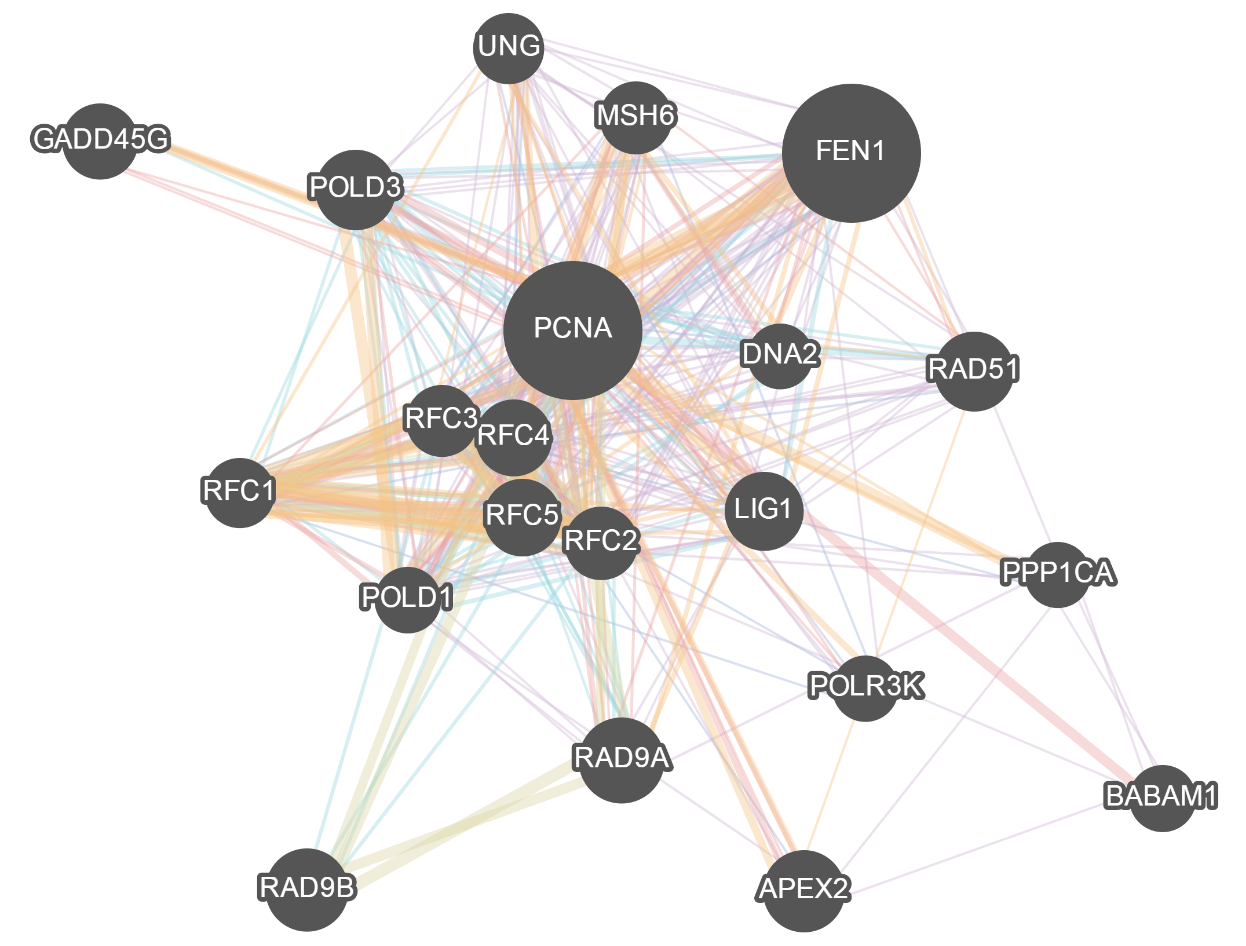
\includegraphics[width=0.7\textwidth]{cytoscape.png}
\caption{Przykład wizualizacji grafu w Cytoscape.js -- krawędzie mogą mieć różny kolor i grubość, pomiędzy wierzchołkami może istnieć wiele krawędzi oraz wierzchołki mogą mieć różny rozmiar}\label{fig:cytoscape}
\end{figure}

\subsection{sigma.js}
\subsection{VivaGraph.js}
\subsection{Linkurious.js}

\begin{table}[H]
\begin{tabularx}{\textwidth}{|r|c|c|c}
\hline 
 & Cytoscape.js & Sigma & VivaGraphJS \\ 
\hline 
Licencja & MIT & MIT & BSD 3 \\ 
\hline 
Rozmiar & 294 & 112,9 & 60,4 \\ 
\hline 
Renderowanie & & & \\
SVG & • & tak & • \\
HTML5 Canvas & • & tak & • \\
WebGL Canvas & • & tak & • \\ 
\hline 
Obsługiwane formaty & • & • & • \\ 
\hline
Rozszerzalność & • & • & • \\ 
\hline 
• & • & • & • \\ 
\hline 
\end{tabularx} 
\end{table}


